%% Section 4 — Structural Dimensions
\section{Structural Dimensions: Ownership, Actor Constellations, and Urban Embeddedness}
\label{sec:structural}

The structural dimension of a CAS, in the Phillips and Ritala (2019) framework, concerns the hierarchy, relationships, and actor constellations that constitute the system's observable architecture. For data center assemblages, this is the dimension that the technical efficiency literature most systematically ignores and that the existing socio-political literature reaches only qualitatively. Who actually owns this infrastructure, in what legal form, and with what consequences for governance? Which actors are constitutive of the assemblage, and through what relationships do they interact? How is the infrastructure embedded in the urban and territorial systems through which it is contested, permitted, and supplied? Work Package 3 addresses the financial and ownership architecture; the city2graph framework \citep{city2graph} provides the tools for the urban-embeddedness layer.

\subsection{WP3: Ownership Cartography and Financialisation}

The question of ownership is not peripheral to the governance dynamics of data center assemblages — it is structural. The dominant ownership form in the world's largest data center market, Northern Virginia's Loudoun County, is the Real Estate Investment Trust. Equinix, Digital Realty, Iron Mountain, and a set of non-traded private REITs collectively control the majority of leasable capacity in the region. The REIT structure is not merely a tax-efficiency mechanism; it is a governance-relevant legal form with direct implications for accountability.

By distributing beneficial ownership across retail investors, pension funds, and sovereign wealth funds, the REIT dissolves the concentrated accountability that would otherwise attach to a single identifiable owner. No single shareholder holds a position large enough to bear reputational or political pressure from local contestation. More consequentially, the operating entity — the colocation provider or tenant REIT — is legally distinct from the asset-owning entity, which is in turn only one fund within a diversified investment vehicle whose beneficiaries are spatially dispersed and, in aggregate, politically inert. When community campaigns, planning bodies, or municipal authorities seek a counterparty capable of making binding commitments about energy sourcing, water use, or capacity limits, the REIT structure provides no such counterparty. The governance surface area — the interface at which political pressure can produce accountable response — has been systematically reduced by a legal form whose primary design purpose is unrelated to planning.

This condition, which we term the \textit{financialisation of digital infrastructure}, is mapped through a pipeline that resolves operator and owner company names from the project's facility index against the OpenCorporates company registry API. For each entity, the pipeline retrieves canonical legal identities, jurisdiction codes, incorporation dates, company type designations, and registered officer networks — a corporate-registry layer that is a prerequisite for the ownership graph, since operating company names frequently diverge from registered names, and holding structures often pass through multiple jurisdictions before reaching an identifiable beneficial owner. The pipeline's output — an auditable trail from facility-index name to registered corporate identity — feeds a network construction step that joins OpenCorporates records, officer data, and REIT asset schedules into a unified ownership graph.

The analytical products of WP3 are two. The first is an \textit{ownership network} in which nodes are legal entities — facilities, operating companies, holding companies, investment funds, and ultimate beneficial owners — and edges are ownership, directorship, and investment relationships. The second is an \textit{actor typology} that distinguishes between vertically integrated operator-owners, colocation operators leasing REIT-held assets, financial asset managers with no operational function, and public or quasi-public entities. These two outputs together constitute the structural map that WP3 contributes: a representation of the hierarchical and relational architecture of the assemblage that makes the governance consequences of ownership form legible.

\begin{figure}[ht]
\centering
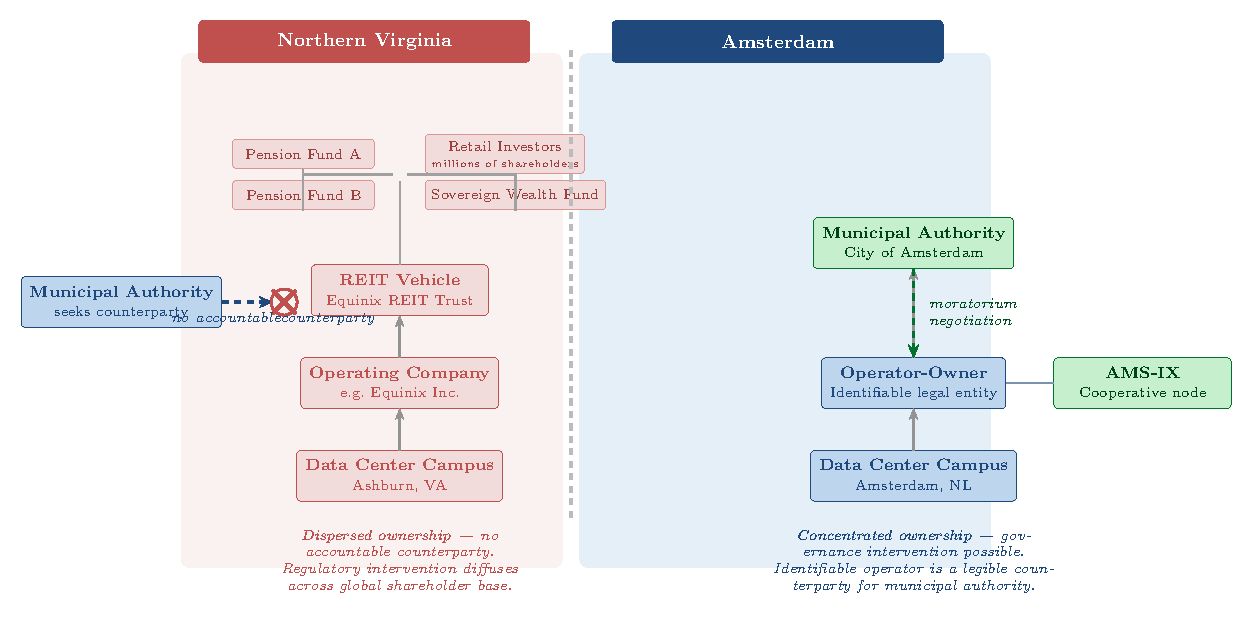
\includegraphics[width=0.92\textwidth]{figures/ownership-contrast}
\caption{Ownership structures and governance capacity: Northern Virginia (REIT-dominated, dispersed) versus Amsterdam (mixed, operator-owned, accountable). The structural difference explains the differential regime response to equivalent contestation intensity.}
\label{fig:ownership}
\end{figure}

The European ownership landscape is structurally different in ways that matter for regime response. Amsterdam's data center market, which experienced a formal moratorium between 2019 and 2022, exhibits a more varied ownership ecology: operator-owned campuses, a cooperative internet exchange (AMS-IX), and sovereign wealth fund investment that, unlike dispersed REIT ownership, is concentrated enough to constitute a visible and accountable actor in governance negotiations. The Netherlands' planning law structures accountability differently, creating clearer channels from municipal authority to identifiable ownership entities. This is not to argue that European ownership structures are uniformly more accountable — US-listed REITs are actively extending their European portfolios, and the structural conditions that make Virginia's governance gap possible are being reproduced in modified form across European markets — but rather that the structural composition of ownership shapes the surface area available for governance intervention in ways the CAS framing makes analytically tractable.

\subsection{Urban Embeddedness and Multi-Actor Constellations}

The ownership cartography of WP3 maps the financial architecture of the assemblage. But the assemblage's actor constellation extends considerably further: to the municipal governments that issue planning permissions, the energy utilities that negotiate grid connections, the water authorities that license abstraction, the residential communities that organise campaigns, the regional transport and land-use planners whose decisions shape what sites become available, and the civic institutions — schools, hospitals, industrial estates — that share the infrastructure on which data centers draw.

These actors are embedded in, and interact through, urban and territorial systems whose spatial structure shapes the possibilities for contestation and governance. The city2graph framework \citep{city2graph} — which converts geospatial urban data into graph structures incorporating infrastructure networks, land use, mobility flows, and spatial proximity relationships — provides the technical basis for representing this embeddedness computationally. Applied to the facility index, city2graph enables the construction of a spatial-relational graph for each jurisdiction in which data center nodes are connected to the urban actors and infrastructure systems they draw on and affect: power grid nodes, water infrastructure, residential zones, transport networks, and the municipal institutions through which planning and governance authority is exercised.

This spatial-relational graph is not merely a background map. It is an analytical object that makes legible the properties of the assemblage that the CAS framing foregrounds: the heterogeneity of actors at multiple scales (from the data center campus to the regional grid to the continental fibre network), the spatial relationships through which contestation is organised (residential proximity, shared infrastructure, political constituency), and the structural differences between jurisdictions that produce different governance outcomes. The comparison of Northern Virginia's low-density exurban geography — in which the data center cluster is spatially separated from residential populations and politically dominant through its contribution to the Loudoun County tax base — with Amsterdam's dense urban-fabric embedding — in which facilities compete for the same land, water, and political attention as residential and cultural uses — is a structural comparison that the city2graph representation makes systematic rather than impressionistic.

A first empirical pass of the pipeline against the project's three seed facilities yields a structurally telling pattern. The script downloads Overture Maps infrastructure and land-use layers for a 2\,km bounding box and builds a heterogeneous graph connecting each facility node to proximate power substations, residential zones, and commercial zones. The Ashburn/AWS facility sits within reach of 36 power-infrastructure nodes --- substations, cables, transformers --- but registers only one residential zone within the 1\,km adjacency radius and zero adjacent-residential edges. The Amsterdam and Dublin facilities show the inverse: the former records 61 residential zones with 16 adjacency edges, the latter 361 zones with 61 edges. The Ashburn profile is not explained by data sparsity: Overture Maps coverage in Loudoun County is comprehensive. It reflects a land-use pattern in which the data center cluster and residential settlement are deliberately separated at the scale of the built environment --- a spatial enactment of the territorial imaginary that makes the infrastructure legible to industrial logistics but invisible to community life (\Cref{fig:urban_embed}).

\begin{figure}[ht]
\centering
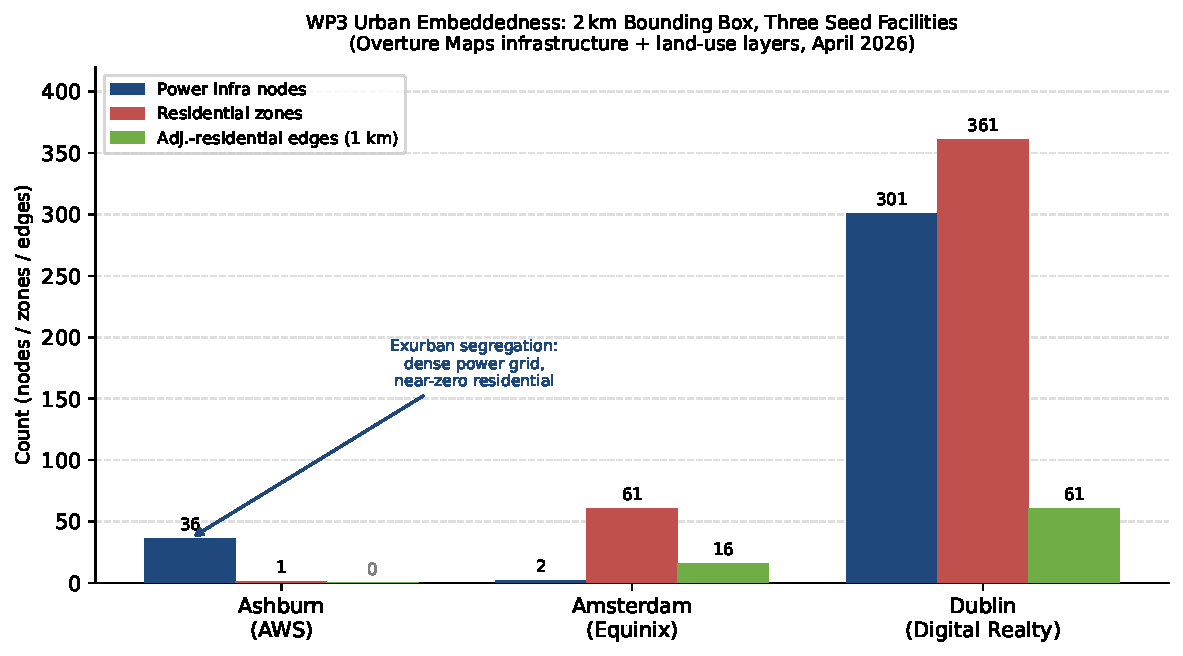
\includegraphics[width=0.90\textwidth]{figures/wp3_urban_embeddedness}
\caption{WP3 urban embeddedness results for three seed facilities (2\,km bounding box, Overture Maps infrastructure and land-use layers). Power infrastructure nodes (substations, cables, transformers), residential land-use zones, and adjacent-residential edges (within 1\,km) per facility. Ashburn's near-zero residential adjacency against its dense power infrastructure profile is a spatial signature of deliberate land-use segregation. Data: pipeline run, April 2026.}
\label{fig:urban_embed}
\end{figure}

\begin{figure}[ht]
\centering
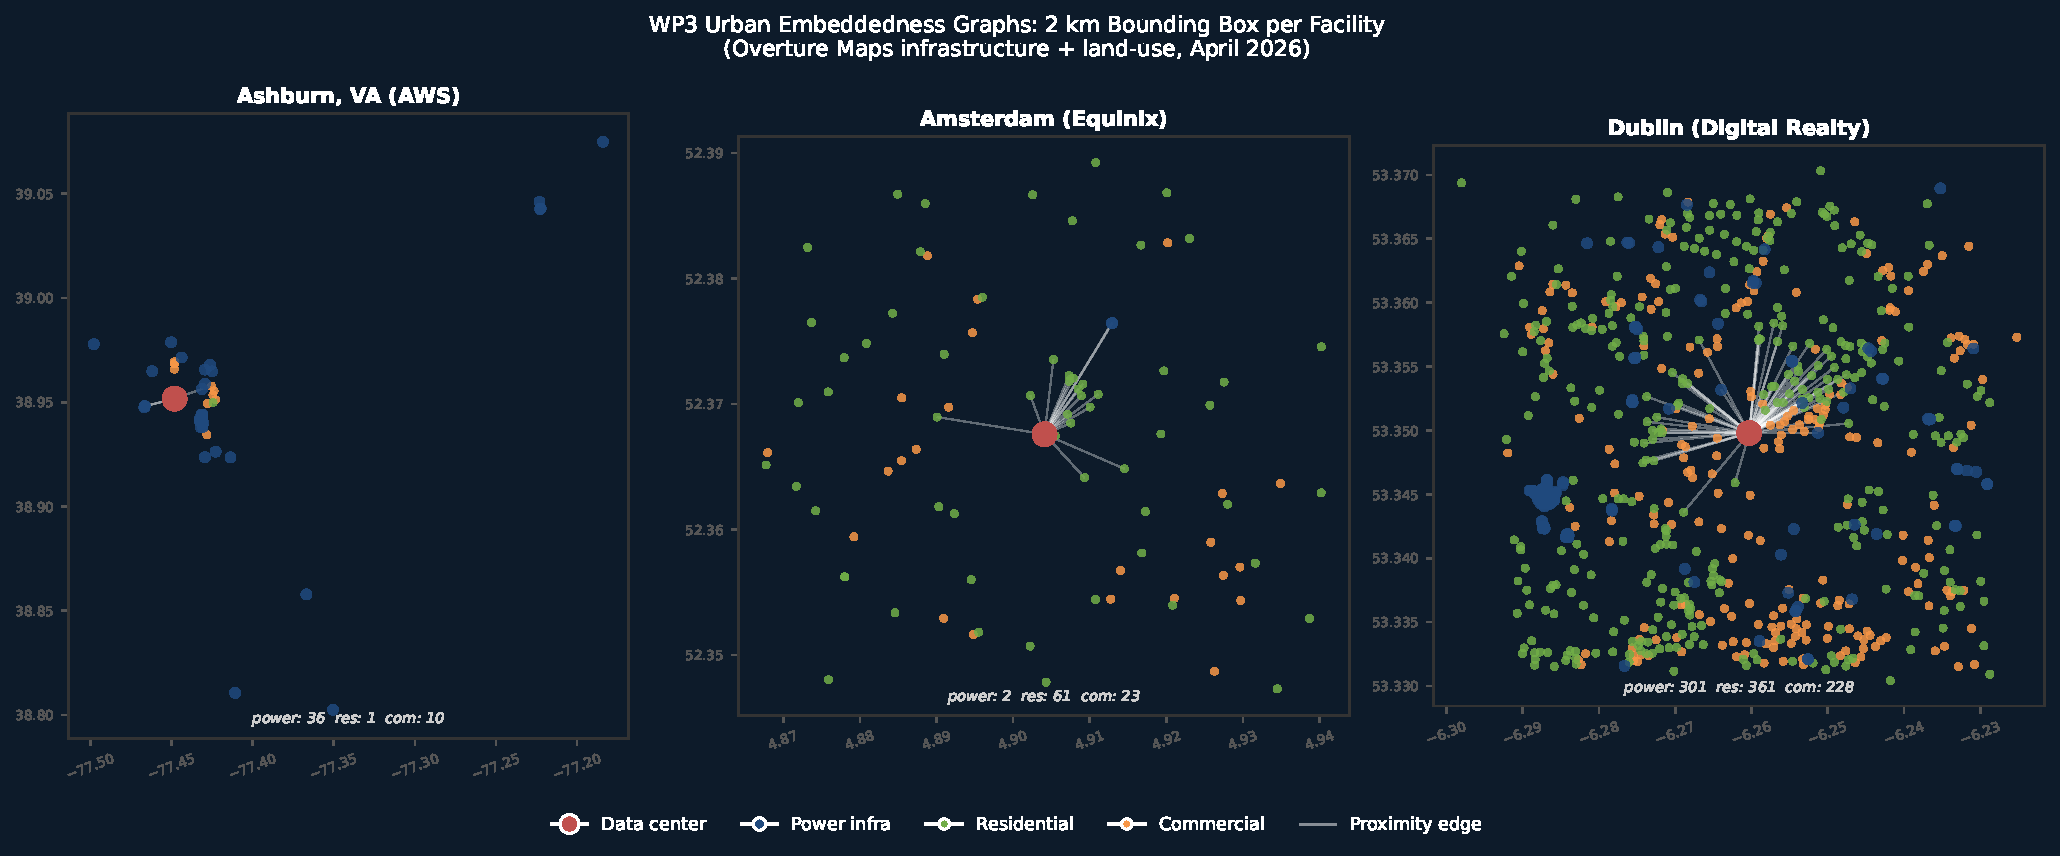
\includegraphics[width=\textwidth]{figures/wp3_urban_graphs_map}
\caption{Spatial urban graphs for the three seed facilities. Nodes are colour-coded by type: data center (red), power infrastructure (blue), residential zones (green), commercial zones (orange). Edges connect the data center to its $k$-nearest power nodes and to all residential zones within 1\,km. The visual contrast between the Ashburn graph --- a sparse residential-edge structure despite dense power connectivity --- and the Amsterdam and Dublin graphs is a spatial representation of the assemblage's embeddedness difference. Data: Overture Maps via city2graph, April 2026.}
\label{fig:urban_graphs_map}
\end{figure}
